\chapter{Agradecimientos}

¿Qué se siente cuando uno echa la vista atrás? ¿Qué es lo que se te pasa por la cabeza antes de pasar la última página de un libro que te ha tenido atrapado horas y horas? ¿Qué queda cuando, en la cima de la montaña, miras hacia arriba solamente para descubrir que todo queda bajo tus pies? Todas las historias acaban de alguna forma o de otra y todo lo que queda cuando lo hacen es el vacío de saber que nunca jamás nada podrá reemplazarlas, ni tan siquiera acercarse a ellas. Es la ineludible sensación de todo aquello que al final del camino ha merecido la pena.

Este documento recoge de forma académica la historia de los mejores seis años de mi vida. Detrás de todos los tecnicismos se encuentra la historia de más de veinte ciudades; de no menos de sesenta vuelos, trenes y coches; y lo más importante: de por lo menos cien personas. Desafortunadamente, no creo que ningún editor con dos dedos de frente decidiera publicar semejante despropósito, de modo que aprovecharé estas páginas que serán publicadas sin revisión para contar mi vida.

Como todo niño fascinado por el espacio, soy un astronauta frustrado. Uno que no tuvo la valentía de moverse y estudiar Física y que por suerte tenía unas manos demasiado sudorosas como para dedicarse a la Arquitectura. El metro ochenta de mi niñez me hizo buen jugador de baloncesto hasta que todo el mundo creció. La portería de fútbol, que será siempre el lugar donde me sienta la persona más importante del Universo, era a la vez demasiado solitaria para mí. Toqué el piano sin brillantez. Pinté sin genialidad. Escribí, publicado, pero escaso de tinta y de imaginación. Diseñé y construí puentes, pero solo de palillos de helado. Probé muchas cosas y tuve la suerte de encontrar mi ikigai en la informática. Supongo que en el momento en el que instalé mi primera tarjeta gráfica y ejecuté \verb|C:\>DOOM\doom.exe| todo quedó sellado. Jamás imaginé que aquel chaval que simplemente quería hacer un videojuego divertido acabaría pasando incontables horas devorando todo el conocimiento que encontrara a su paso sobre programación, estructuras de datos y algoritmos.

Así pues, como toda mi generación, entré en la Universidad con la promesa de un empleo y una vida digna ganada gracias al estudio. Transcurrieron así los mejores momentos de mi vida entre partidas de futbolín, preocupaciones y caras de sueño antes de entrar a clase, risas al salir de ellas y noches de partidas eternas de League of Legends y Counter Strike. Nada tiene que ver la persona que entró (cerrada, de frases cortas y sonrisas escasas) con la que salió (decidida, locuaz y risueña). De paso, conseguí vestirme de una manera algo más decente, aunque sigo sin encontrar la manera de combinar colores con acierto. En esos cuatro años conocí a un grupo de personas excepcionales, aprendí y estudié hasta el más mínimo detalle, me encontré con quienes serían mi guía en los años venideros y descubrí que la investigación era mi misión en la vida.

Al terminar, volé por primera vez por mi cuenta hacia el Centro de Supercomputación de Jülich (Alemania) para lo que sería mi primera estancia fuera. Fueron sin lugar a dudas el momento más trasdencental en mi vida. Tan buen recuerdo guardo de aquellas semanas que nunca quise volver por no estropearlo. Como diría el maestro Sabina: "[...] que al lugar donde has sido feliz, no debieras tratar de volver [...]".

Más por inercia e ilusión que por lógica, decidí estudiar un máster en Automática y Robótica en mi alma mater. Siendo sinceros, no fue la alternativa más inteligente para mi futuro (no por el máster en sí). Sencillamente, con el paso del tiempo me di cuenta de que en el fondo siempre me arrepentiré de no haber subido a un avión para descubrir otra Universidad. Sin embargo, de no haberme quedado, jamás habría conocido tanto ni hubiera trabado amistad con una de las mejores personas que se han cruzado en mi vida. Cada vez que pienso en que tendría que haber volado, le recuerdo comiendo un limón entero con piel y se me pasa.

Como si de alguna forma se escucharan mis lamentos, la vida me dio la oportunidad inmejorable de volar hacia los Estados Unidos e investigar en una de las compañías a las que más cariño guardaré. Así acabé viviendo en Mountain View (California) y trabajando para NVIDIA con un equipo excepcional. Fueron meses de descubrimiento y quedarán para siempre en mi memoria los recuerdos de mi pequeña habitación en Villa Street, del conductor de autobuses al que nunca le pregunté su nombre pero que siempre me llevaba con una sonrisa al trabajo y un "Hey, buddy!", de las partidas de ping pong, del DeLorean aparcado delante de mi casa y de disfrutar de los Juegos Olímpicos en el proyector de la casa de Cole gritando "USA, USA, USA!". La hospitalidad de Cole y Grayson hicieron que esos meses se me pasaran volando.

\newpage

Como el hombre es el único animal que tropieza dos veces con la misma piedra, regresé de nuevo a Alicante a comenzar mi doctorado. De nuevo, uno de mis mayores defectos me jugaba una mala pasada y nublaba mi juicio al elegir: la comodidad. De nuevo, siempre quedará en mi cabeza la incógnita de qué hubiera ocurrido si hubiera decidido quedarme en Estados Unidos en lugar de volar de vuelta. De nuevo, como si algún desconocido bondadoso me ayudara a llevar una carga pesada, la vida se encargaría de darme una palmada en la espalda y recordarme que no fue tan mala elección. Apenas unas semanas después de mi vuelta, quizás movido por la confianza insuflada por todo lo conseguido, quizás guiado por la inconsciencia etílica, envié un mensaje que me permitió conocer a la persona que me ha dado todo lo que me faltaba en la vida. Como un Tetris perfecto, todas las piezas empezaron a caer en su sitio: con la guía y el empuje de mis directores (más amigos que jefes) y con el regreso de viejos compañeros formamos un equipo con el que con mucho esfuerzo conseguimos empujar mínimamente la frontera del conocimiento pero con el orgullo del trabajo bien hecho pese a todos los obstáculos. De nuevo, con la fortuna sonriendo, partí una vez más hacia Estados Unidos a trabajar con una de las personas que más admiraba desde que comencé mis andaduras. Fue un otoño complicado, con mi cabeza más dispersa que nunca y marché con la sensación de no haber hecho todo lo que estaba en mi mano.

Esa cabeza dispersa pasó unos cuantos meses más perdida y con la sensación de estar desperdiciando el tiempo. La inevitable comparación con todo el mundo alrededor del globo no era favorable. Las experiencias vividas, si bien enriquecedoras, eran un arma de doble filo capaces de minar la confianza en uno mismo al darse cuenta de todo el talento y la gente excepcional que trabaja sin cesar fuera. La perspectiva del fin de la etapa añadía todavía más si cabe un componente de incertidumbre que se transformó en sueño escaso, irritabilidad, desmotivación y pesimismo. Me convertí en mi propio peor enemigo, incapaz de sentirme satisfecho con el pasado, completamente ajeno del presente y ciego de cara al futuro. Avanzando a rastras, buscando refugio en todos los hobbies existentes (muchos de los cuales se acabaron convirtiendo en una decoración fantástica para mi habitación) y únicamente espoleado por los estudios paralelos en Física y por el aliento de los seres queridos para continuar, comencé a escribir el documento que aquí presento.

\newpage

Fue justo en el momento de mayor desánimo en mi carrera cuando ocurrió algo completamente inesperado que lo cambió todo. Sin ninguna gana ni motivación, partí hacia Zürich a pasar los meses de verano en la que sería mi última estancia, de nuevo en Oculus. En el momento en el que más lo necesitaba, todos los astros se alinearon para ofrecerme una ciudad y una casa fantásticas, un equipo de gente extremadamente capaz y amigable, un mentor atento y comprensivo... y un grupo de gente de mi tierra tremendamente afín con el que compartir absolutamente todo. Gracias a ello recuperé la motivación y la ilusión para seguir adelante y poder escribir estas líneas.

Como podéis leer, ha sido un camino curioso y lleno de subidas y bajadas. Esta montaña rusa emocional me ha costado pelo, horas de sueño, discusiones y muchos arrepentimientos. Sin embargo, ahora en pie desde la cima de la montaña, observando mi vida a vista de pájaro puedo decir que no hubiera cambiado nada. He recorrido mi propio camino toda la honestidad e integridad que he podido, he volcado todo el esfuerzo que mi salud mental me ha permitido y he tratado de ser la mejor versión de mí mismo a cada paso dado. En algunas ocasiones habré acertado y en otras habré fracasado, pero este ha sido el camino que yo he trazado y eso es algo que recordaré con cariño toda la vida.
Ante mi vista se extienden ahora innumerables cumbres que antes jamás hubiera podido divisar ocultas por las nubes a gran altura. Aquí planto mi bandera y me siento a agradecer a todas aquellas personas que de alguna forma o de otra me han permitido llegar hasta aquí.

Gracias a todos aquellos profesores que se esforzaron en su día a día lleno de complicaciones para que sus alumnos aprendieran y que día a día nos demostraron su cariño y su implicación. Estoy seguro de que si alguno de vosotros tanto del Colegio Sagrada Familia como del Colegio El Valle leéis estas líneas os sentiréis identificados y van por vosotros. En concreto, quiero dedicar unas líneas a agradecer a una persona excepcional que tendrá siempre mi más profunda admiración: Don Carlos. Más allá de enseñarnos, supo transmitirnos pasión, autenticidad y cariño hasta en los días más difíciles. No puedo olvidarme tampoco de Don Francisco, de quien aprendí la importancia del lenguaje; si algún día escribo una novela, será culpa suya.

\begin{center}
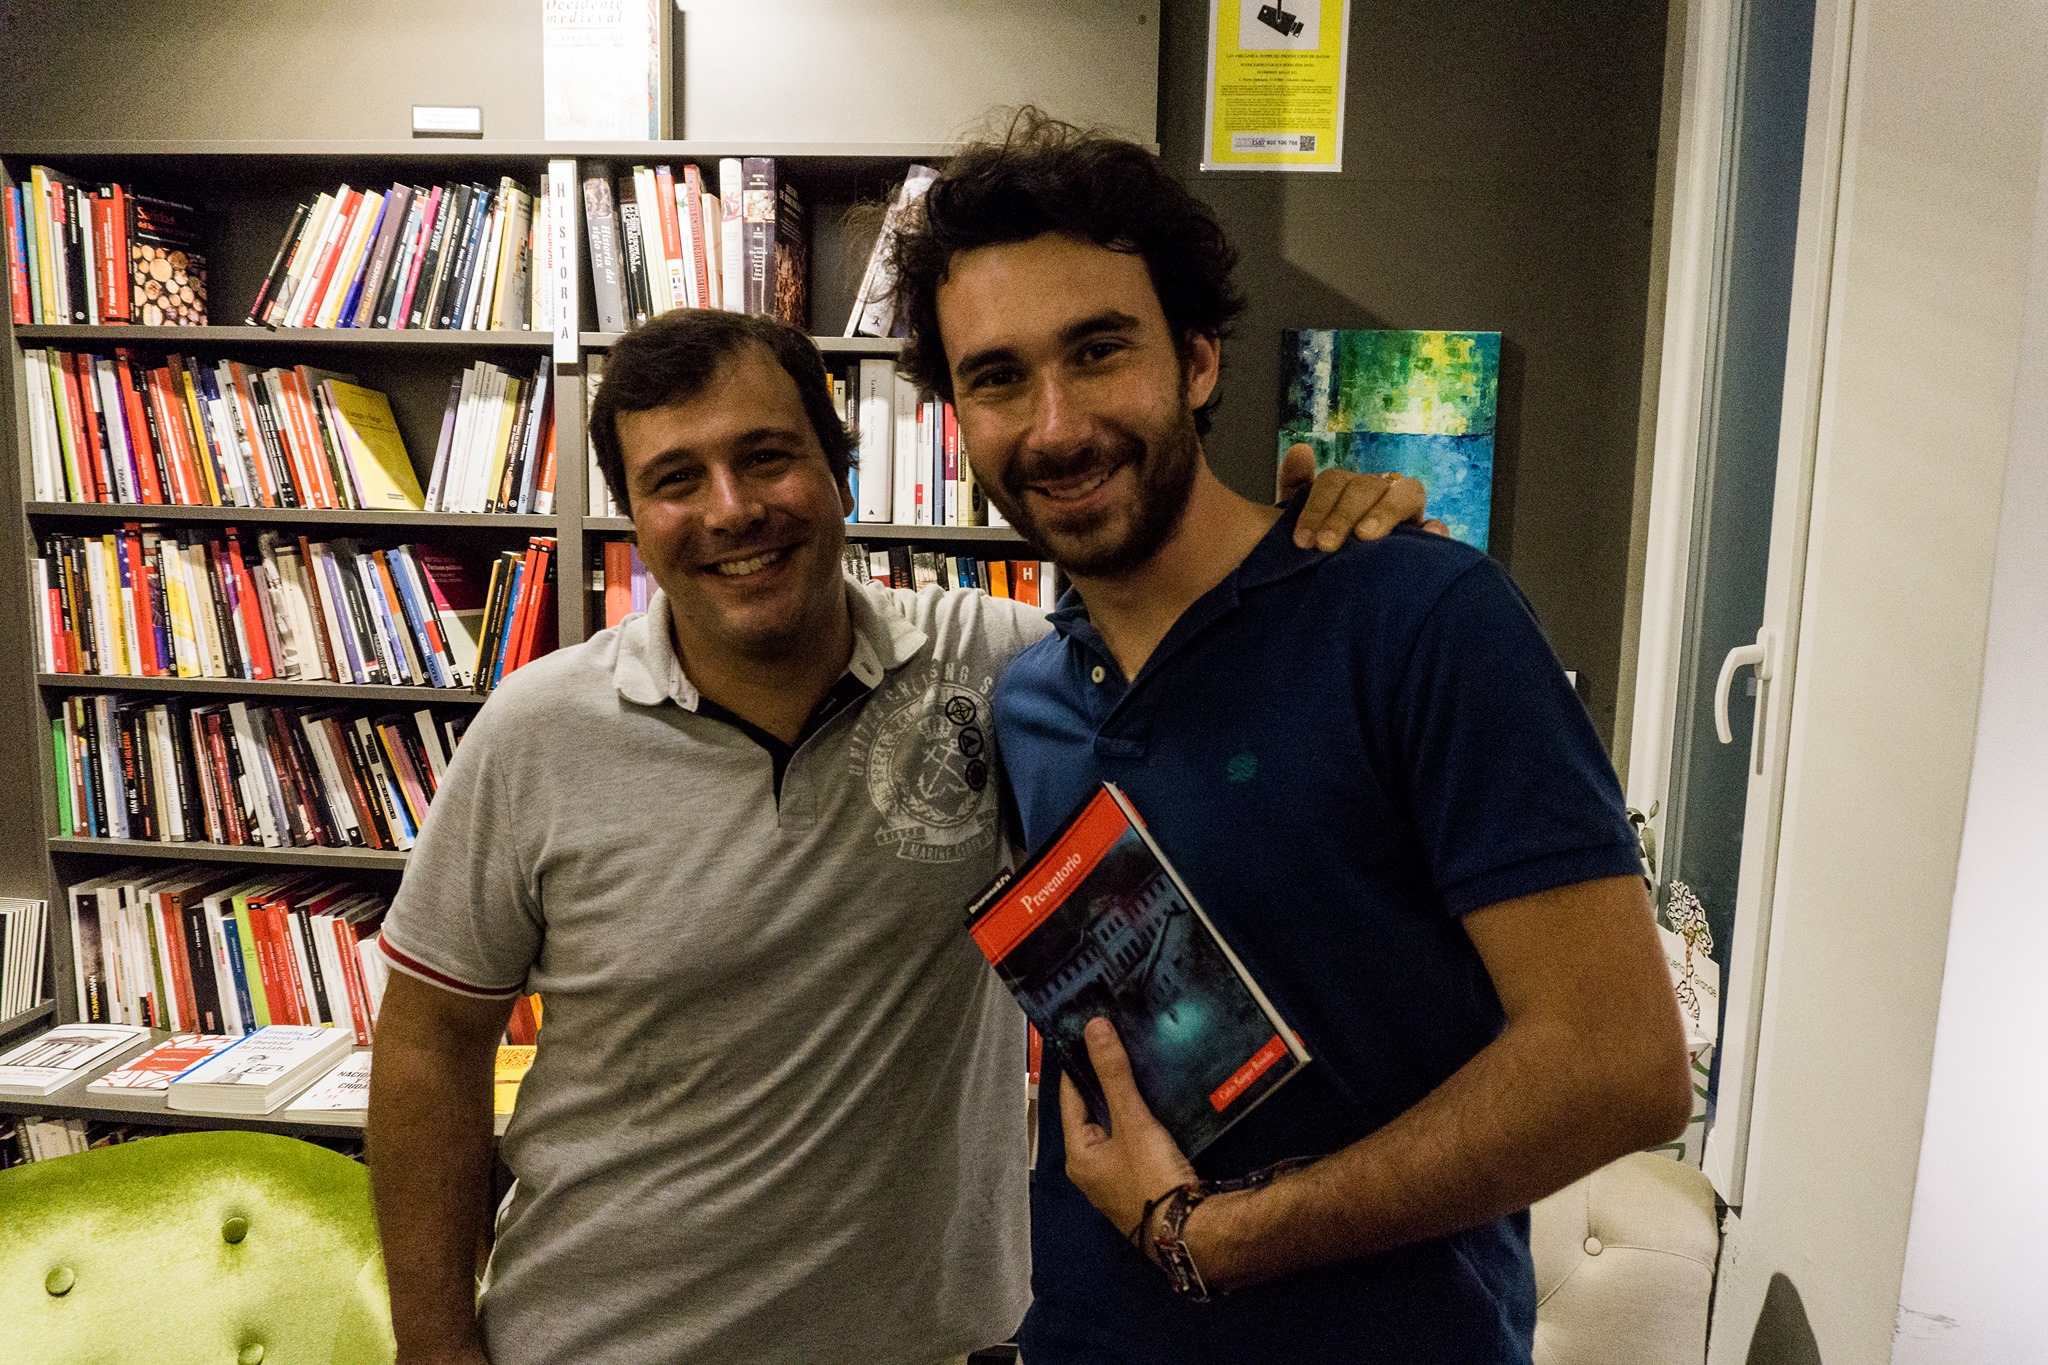
\includegraphics[width=0.7\linewidth]{Figures/Ack/valle2}
\end{center}

Gracias a todos los profesores universitarios que, rodeados de incompetencia, obstáculos y desgana, siguieron dando todo lo que tenían para mantener la educación pública en el lugar que se merece. Aprovecho estas líneas para agradecer a José Miguel Torrejón por demostrarnos que lo difícil se puede hacer fácil con la explicación adecuada y por tener siempre su puerta abierta para cualquier curiosidad. De la misma manera a José Pons, por hacer todo lo que estuviera en su mano para que pudiera formarme en Física y ofrecerme una nueva oportunidad que explorar.

Gracias a todos aquellos que fueron mi guía durante mi etapa investigadora. A Higinio porque realmente él es el responsable de que me dedicara a investigar, gracias por tu franqueza, dedicación y sinceridad.

A Jose, por acogerme y tratarme siempre como un amigo; aunque no hayas estado en la arena, has peleado por mí y siempre has tratado de buscar lo mejor para mi futuro incluso cuando lo mejor para mí no era lo mejor para ti; no has sido mi director, has sido mi amigo y padre académico.

A Sergio, porque sin él todo lo conseguido hubiera sido directamente imposible; has estado con todos nosotros siempre al pie del cañón no importa cuándo ni dónde, has sido el pegamento que nos ha mantenido unidos, el espejo en el que todos nos hemos querido mirar y la fuente de inspiración que nos ha empujado a todos a ser mejores cada día.

\begin{center}
	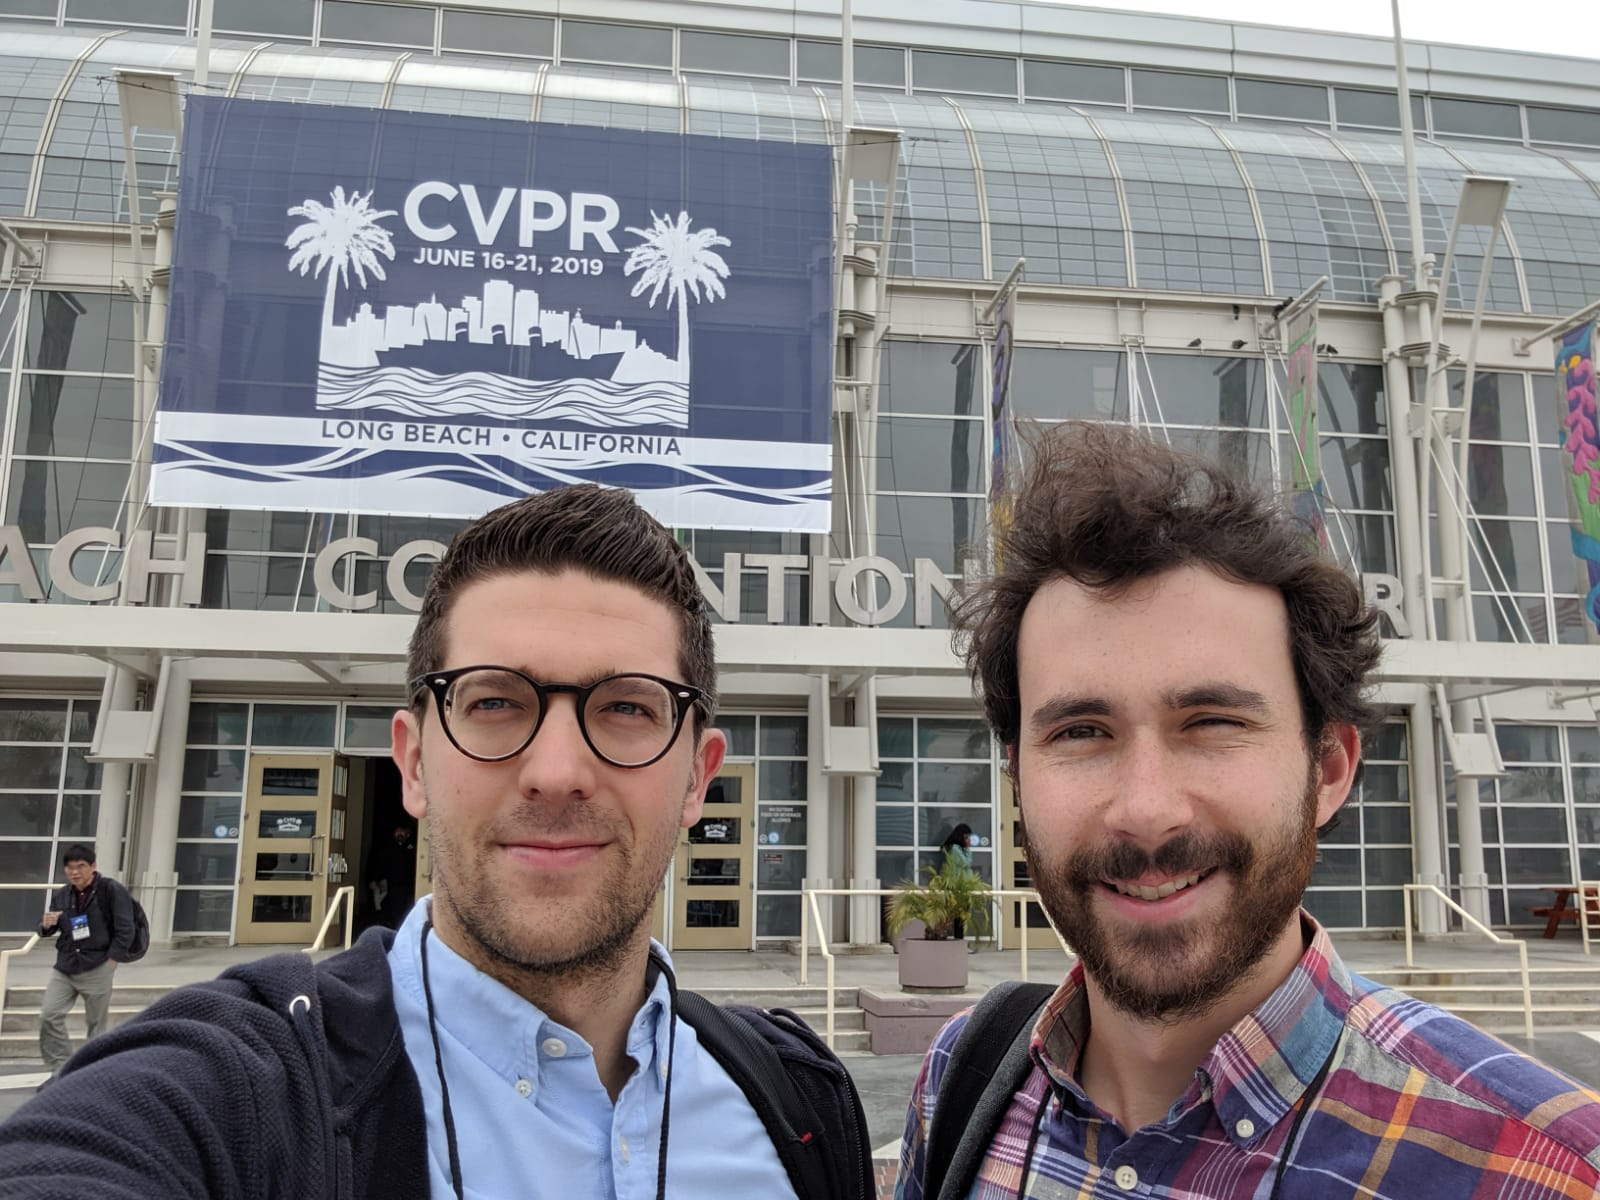
\includegraphics[width=0.6\linewidth]{Figures/Ack/sergio}
\end{center}

A Ivo, porque su energía es contagiosa y su optimismo incansable. A David, aunque de él solo puedo decir lo contrario.

A mi mánager y mentores en NVIDIA, Howard, Bryan y Shalini, por todo el tiempo que me dedicasteis y el buen trato que recibí de vosotros. A todos los integrantes de NVIDIA Research y del equipo de Camera Solutions por compartir tanto conocimiento y consejos: Orazio, Kihwan, Jinwei, Pavlo, Jan, Vidya, Dhaval y John. A todos los interns que compartimos tantos buenos ratos, preocupaciones y naps: Suren, Robert, Behrooz, Zhaopeng y Abhishek.

\begin{center}
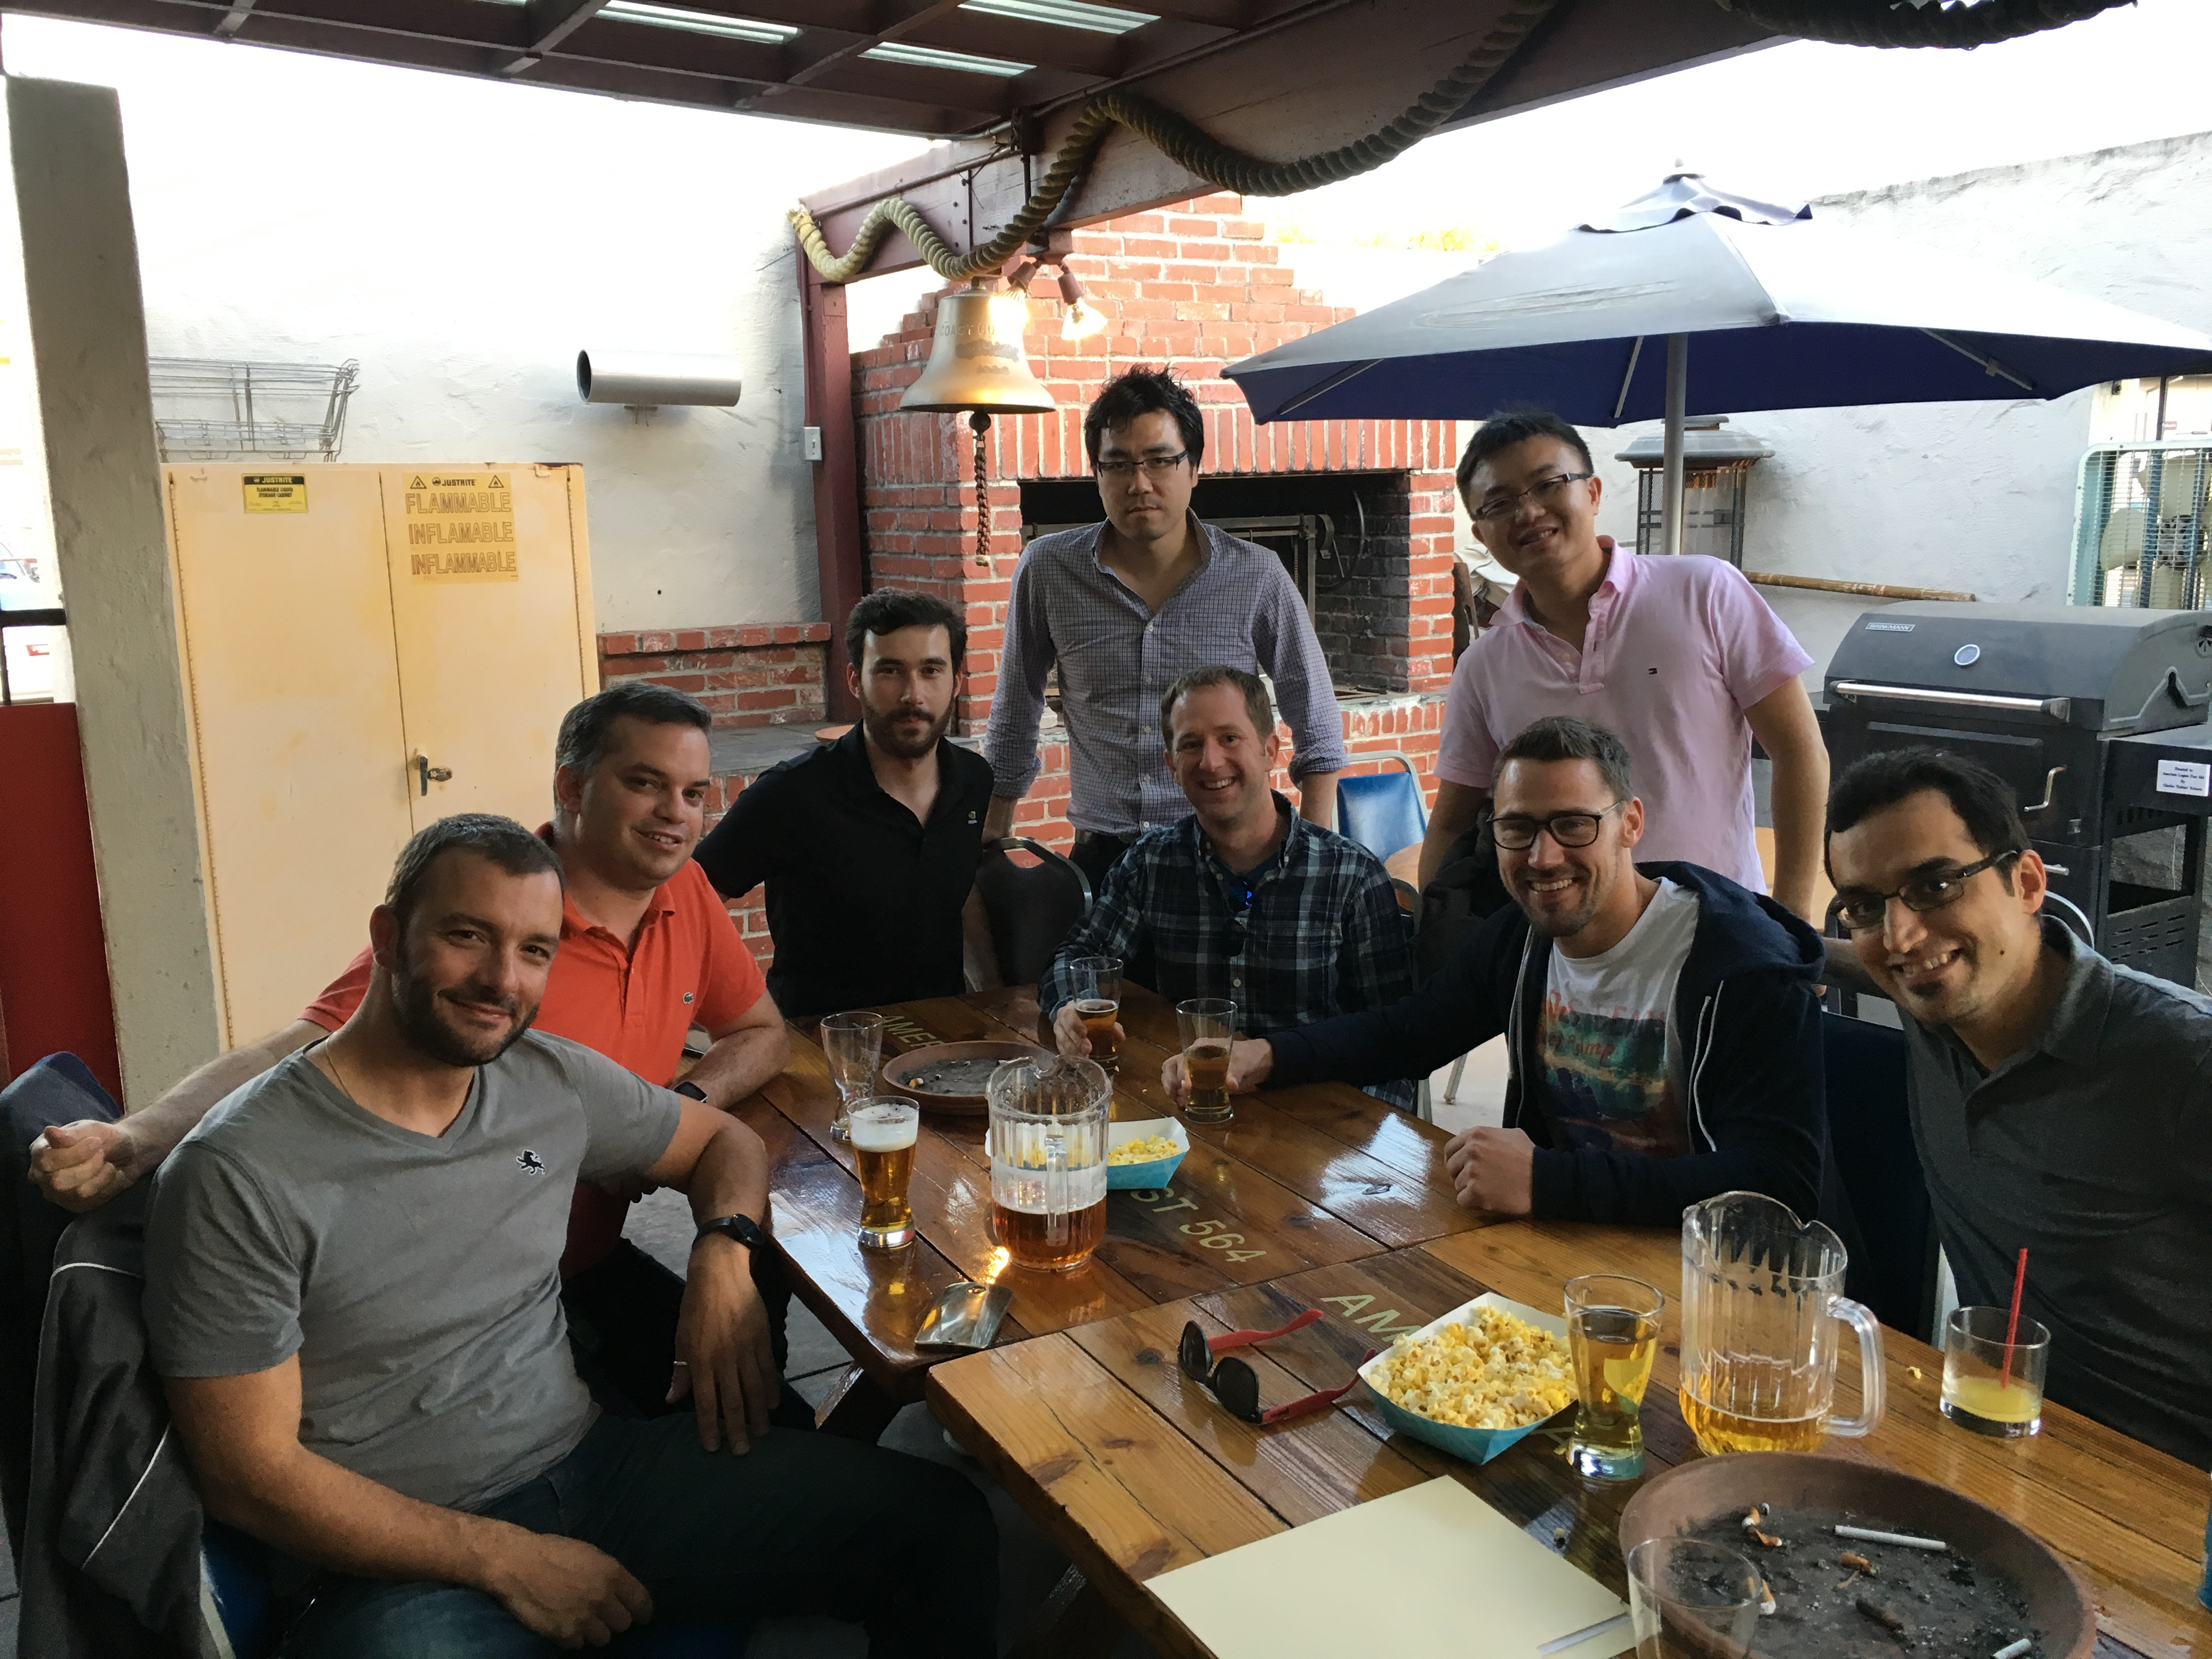
\includegraphics[width=0.44\linewidth]{Figures/Ack/nvidia}
\includegraphics[width=0.5\linewidth]{Figures/Ack/nvidia2}
\end{center}

A mi mentor durante mi estancia en Facebook Reality Labs, Richard Newcombe, para mí fue alucinante poder compartir ideas con alguien al que admiraba tanto, gracias por hacer un hueco en tu agenda. A Raúl por hacerme más llevadera la estancia. A Lingni por tener tanta paciencia conmigo, jamás he visto a alguien que trabaje tan duro. A Svet por sus archivos de calibración. A los demás compañeros del equipo Surreal y Oculus Research que me hicieron sentirme como en casa: Nikki, Theo, Julian, Carl, Tom y Steve.

\begin{center}
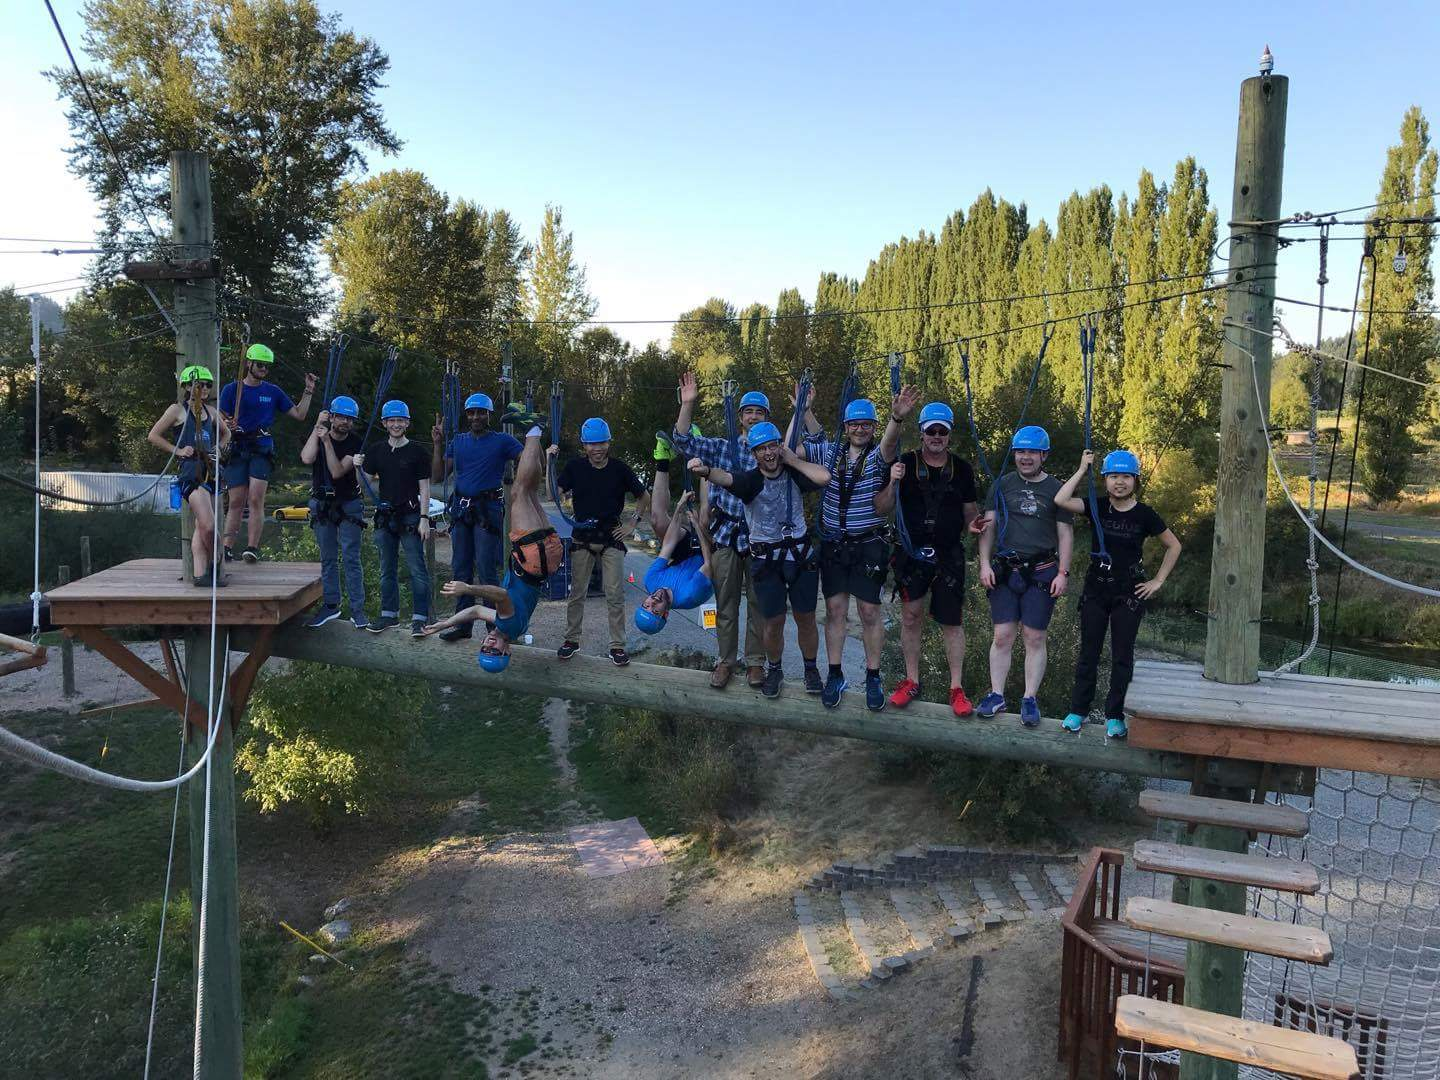
\includegraphics[width=0.6\linewidth]{Figures/Ack/frl2}
\end{center}

A los alumnos con los que he tenido el placer de compartir algunas horas. Gracias por darme vuestra atención y cariño. Nunca imaginé que disfrutaría tanto de la docencia pero os puedo asegurar que con vosotros en el aula he compartido algunos de los momentos en los que me he sentido más lleno en la vida. En especial, gracias a todos los que decidisteis invertir vuestro tiempo conmigo haciendo vuestro TFG o prácticas: Álvaro, Adri, Alexei, Iván, Plácido, Mario, David y Pablo. Vuestra curiosidad y empuje me hacían tener ganas de veros cada día. Espero que todos consigáis todo lo que os propongáis y lo compartáis conmigo allá donde andéis.

\begin{center}
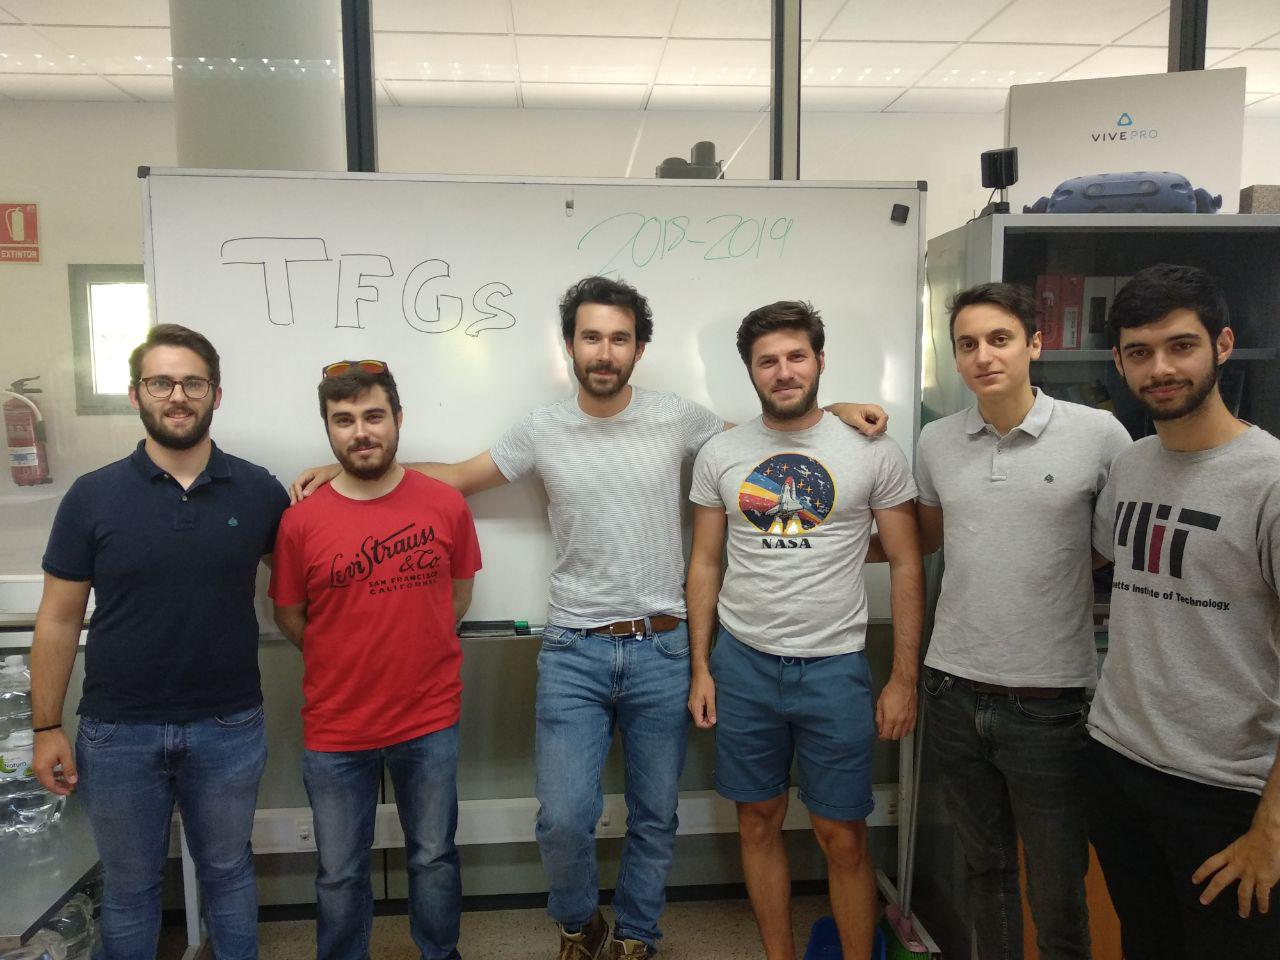
\includegraphics[width=0.64\linewidth]{Figures/Ack/tfg1}
\end{center}

A todos los personajes célebres que han pasado por el laboratorio y que de alguna forma o de otra han aportado su granito de arena para hacer los días diferentes: Rafa, Marcelo, Jose María, Luis, Vicente, Alexandros, Zuri, Isaza, Alejandro, Pau, Toni, Jose Manuel... Y a Joan Carles por dar de alta mi dirección MAC y enseñarme a jugar al pádel.

\begin{center}
	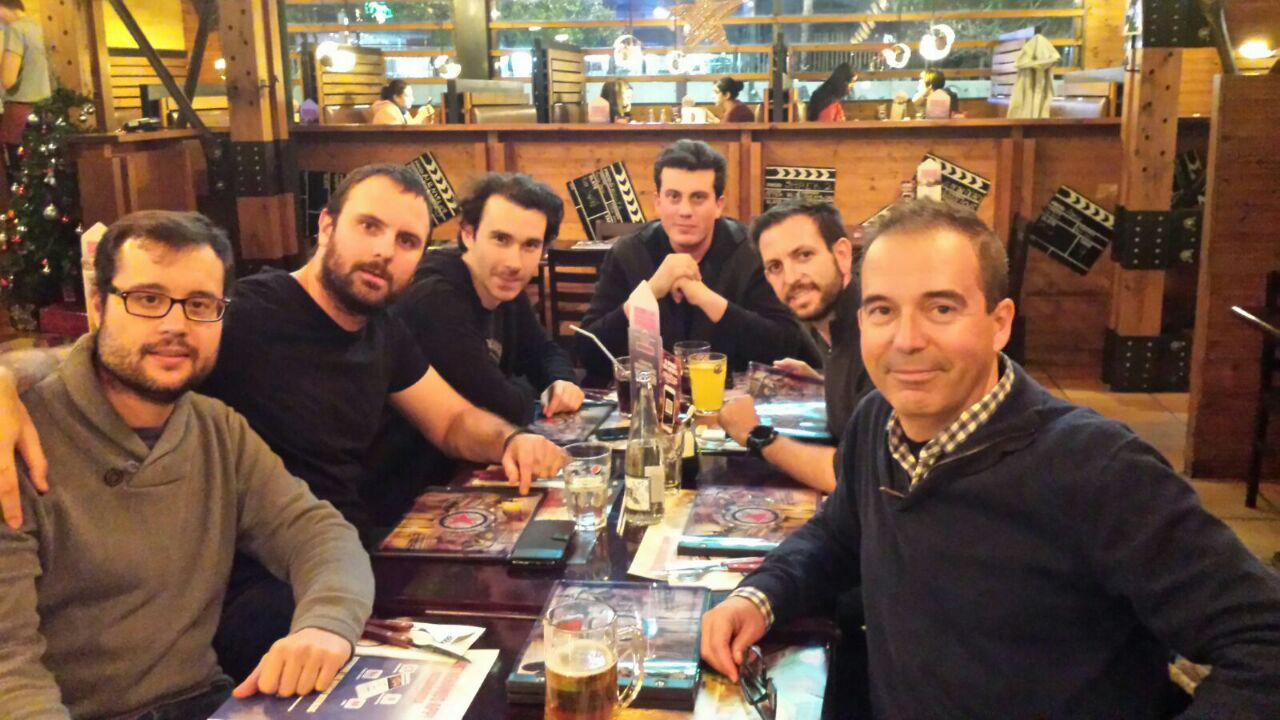
\includegraphics[width=0.75\linewidth]{Figures/Ack/dtic1}
\end{center}

A todos los compañeros inolvidables que he tenido el placer y la suerte de conocer durante la carrera, en el preciso orden en el que saludé a cada uno de ellos: Manu, 0xthor, Pajarraco, Mmarinero, Pable, Víctor, Ginés, Caye y por último y no menos importante, Brayan. Jamás en la vida volveré a encontrar un grupo de gente con la que compartir tantas aficiones, risas, cafés, noches en vela y rusheos por B. Todo lo que pudiera escribir aquí se quedaría corto.

\begin{center}
	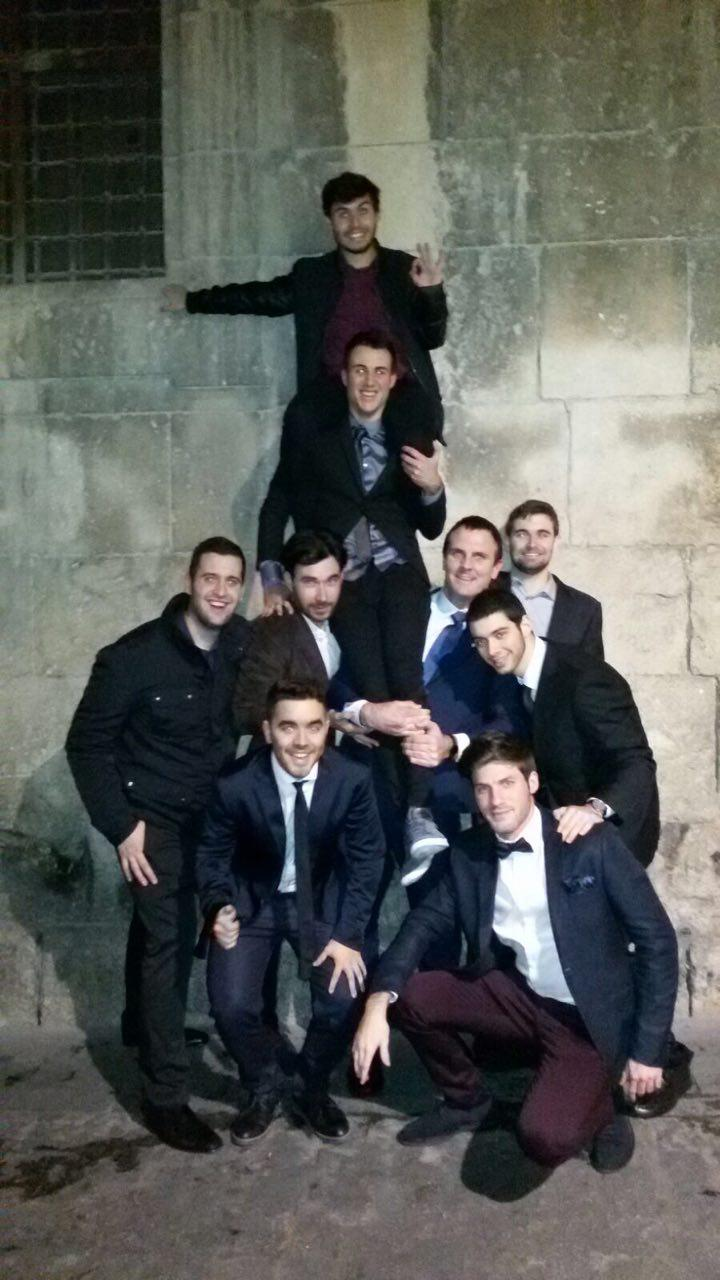
\includegraphics[width=0.5\linewidth]{Figures/Ack/bsc1}
\end{center}

A mis compañeros de isla de investigación: Pable, Sergiu y John. Por demostrar que cuando remamos todos juntos sin quejarnos podemos hacer lo que queramos y llegar hasta San Sebastián.

\begin{center}
	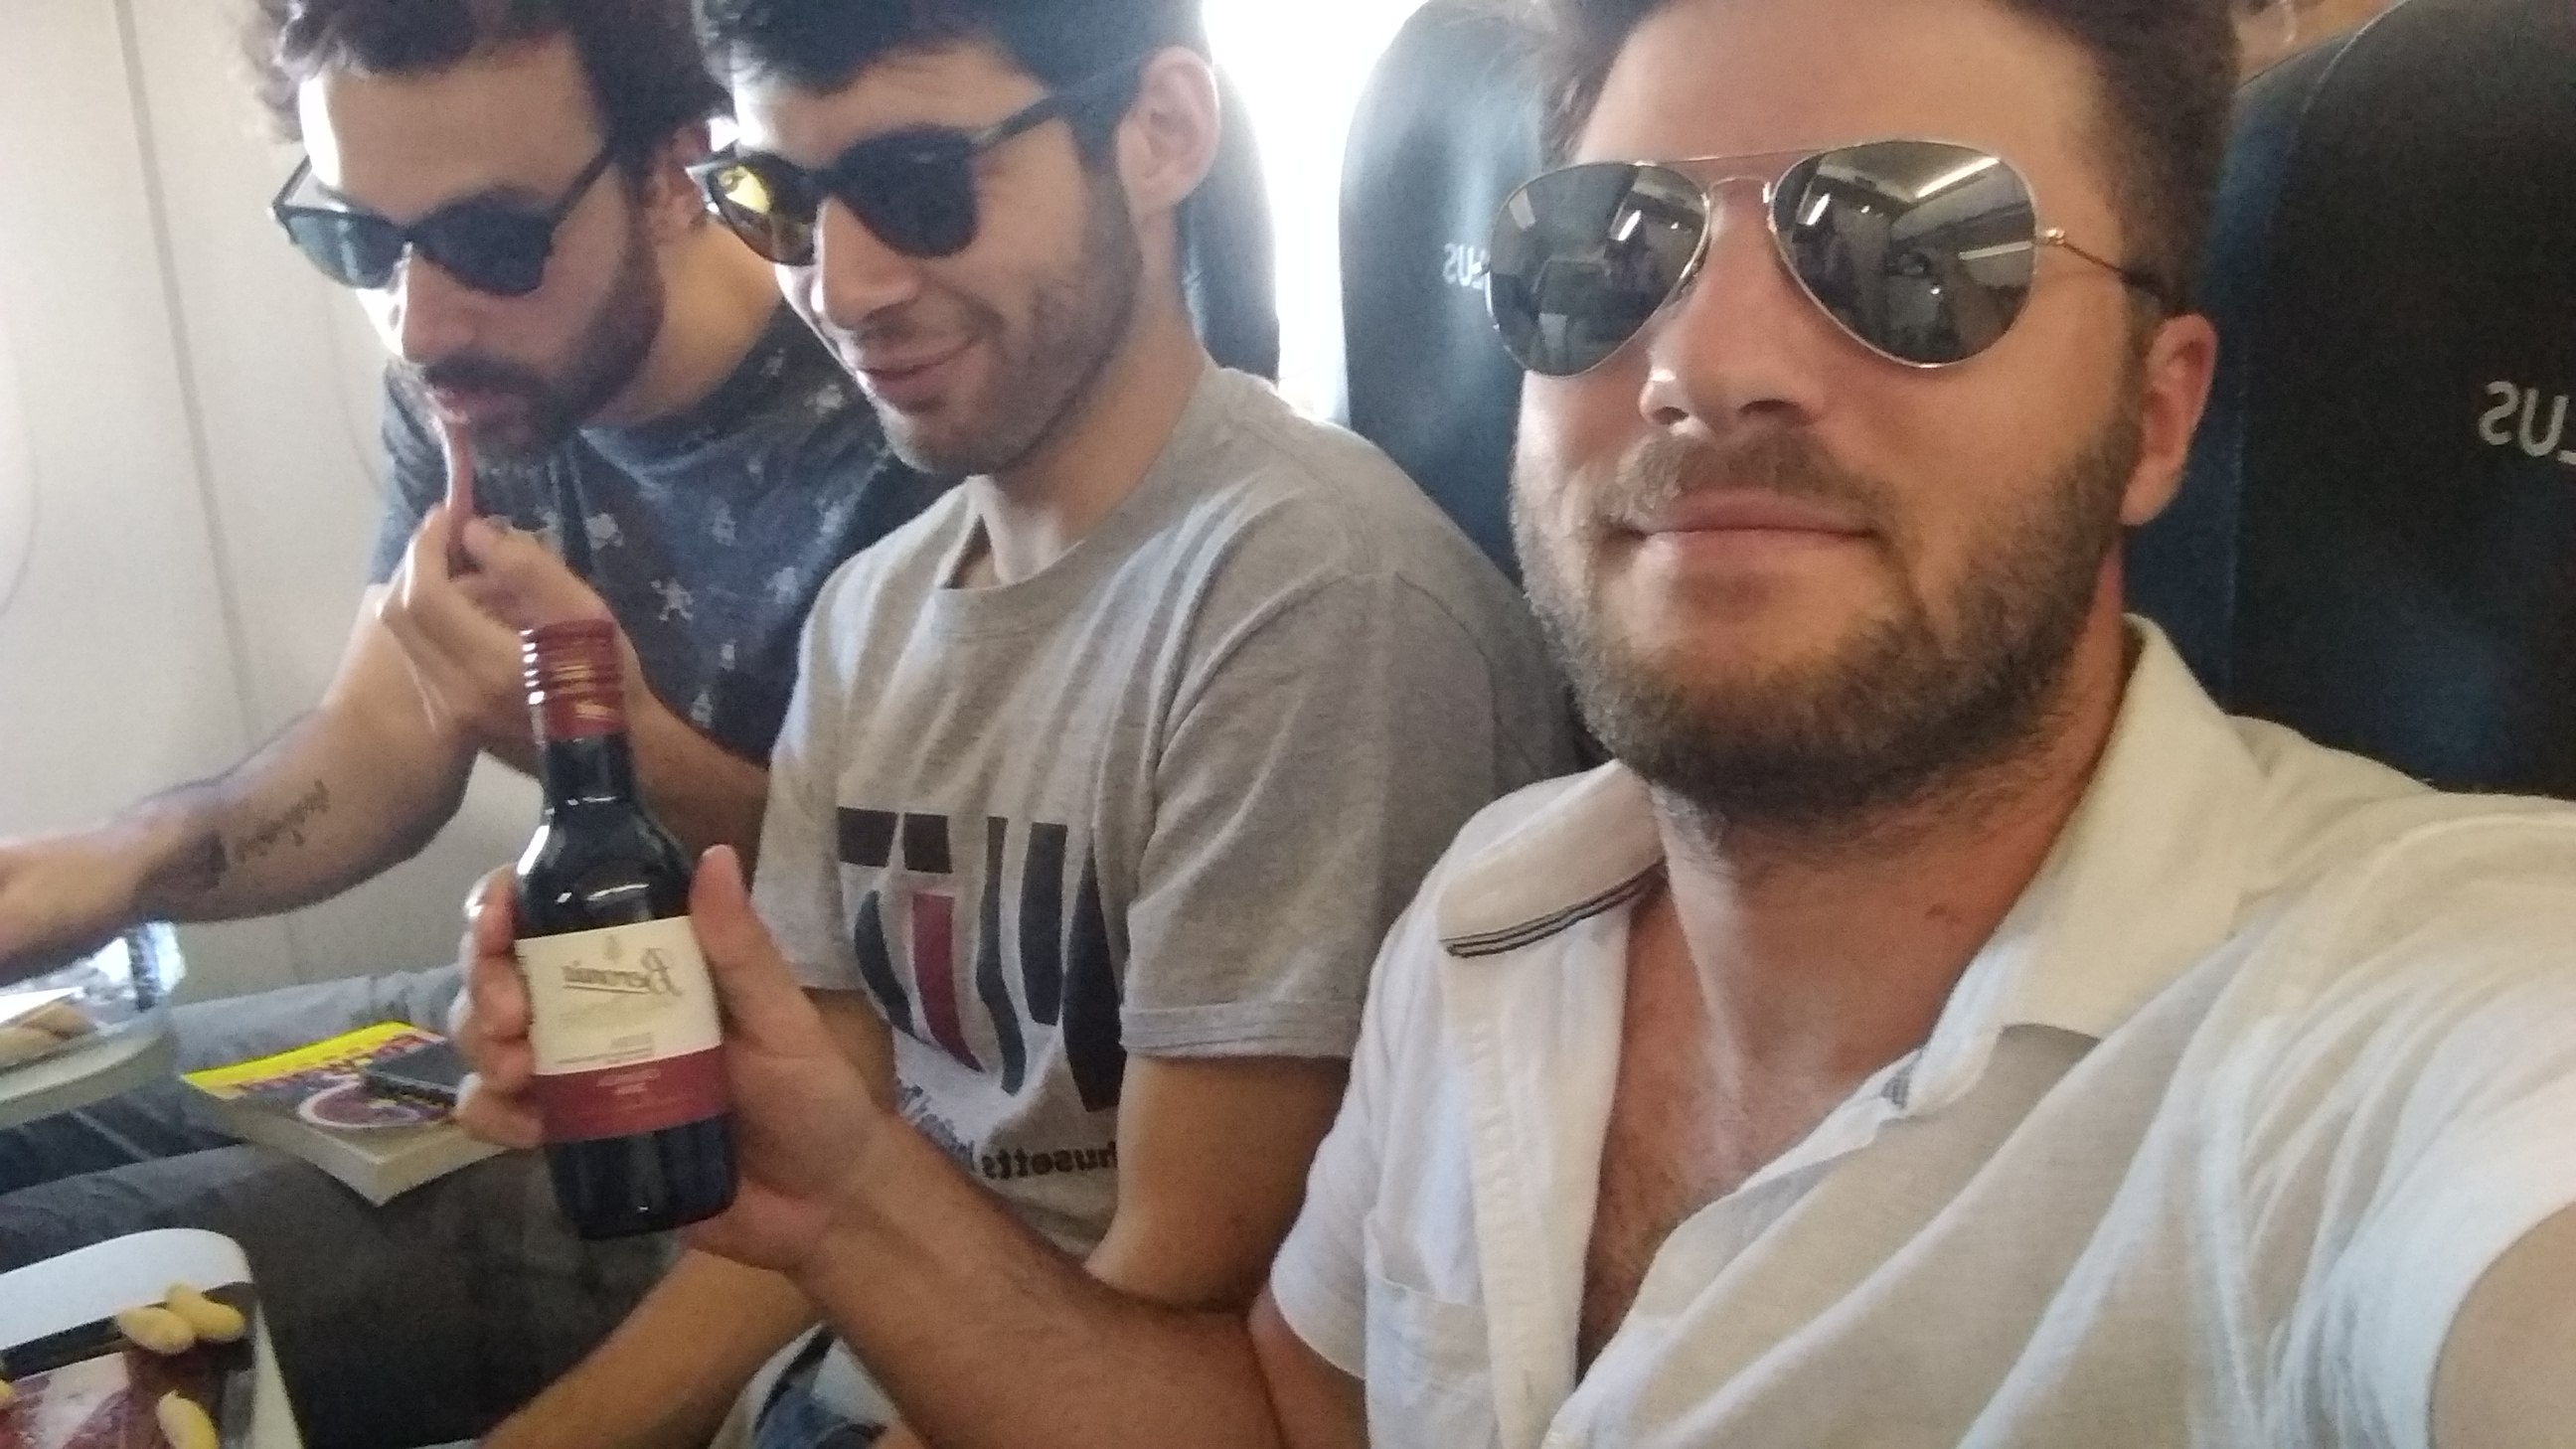
\includegraphics[width=0.7\linewidth]{Figures/Ack/st1}
\end{center}

A mis dos compañeros del máster: Víctor y Fran. Por todas las penas y todas las risas compartidas en la etapa más deprimente y vacía de mi vida. Dudo mucho que hubiera podido terminarla sin la sinergia de estos dos grandes tipos: un nihilista irreconducible y un bonachón inquebrantable.

\begin{center}
	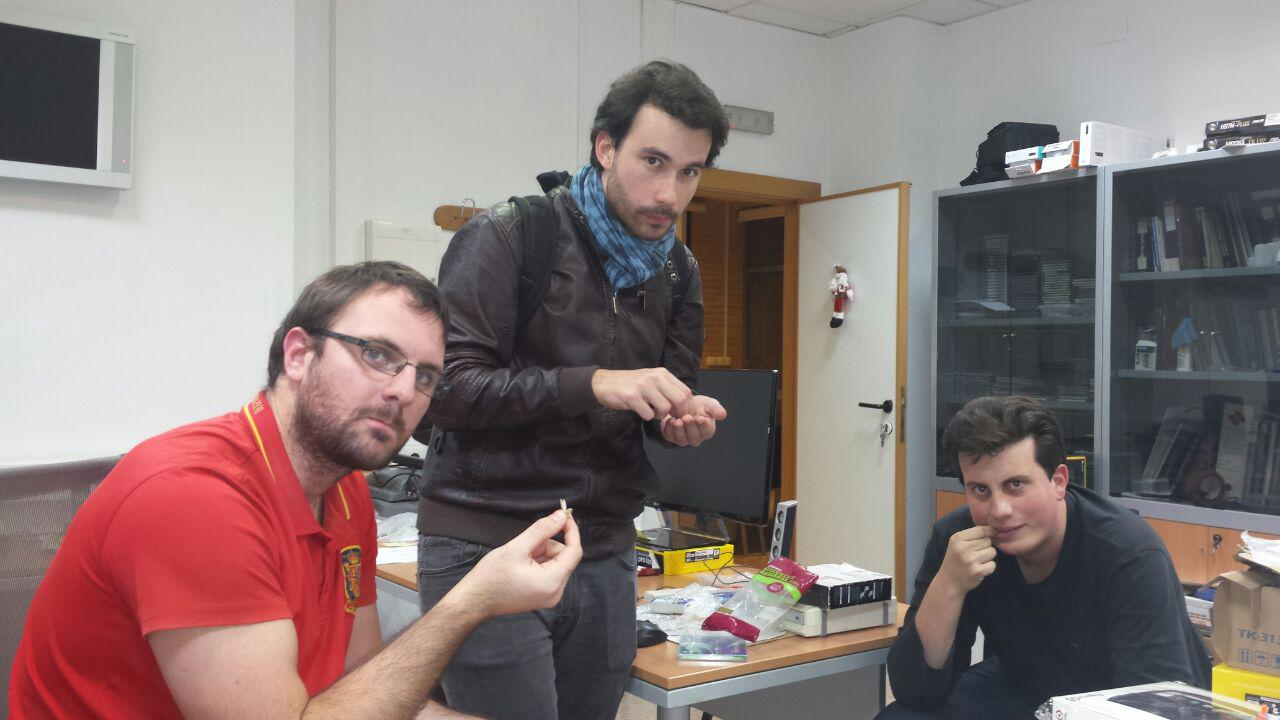
\includegraphics[width=0.7\linewidth]{Figures/Ack/mayr}
\end{center}

A toda la gente de Zürich que me hizo recuperar la ilusión y la motivación en mi trabajo. A mi mánager, Diego Tipaldi, por su amabilidad, comprensión, su capacidad para alegrarse de todas las pequeñas victorias y por su incansable empeño en conseguir que todo el equipo se sintiera a gusto. A toda la gente de mi equipo, de la oficina y de otros lugares del mundo que acudieron en mi ayuda sin pensárselo dos veces: Chino, James, Amy, Jan, Alex Sorkine, Gaurav, Manuel, Alex Locher, Alexandru, Paul, Micky, Mahdi y Nikita. A los demás interns que compartimos muchas cenas gratis los lunes y los jueves: Katrin, Joao y Audrey. A todo el equipo de recruiting: Tanja por estar siempre atenta a nosotros, Oliver por suministrar siempre pasteles y Leslie por el tecno.

A la Spanish Mafia. Máximos responsables de que los meses en Suiza sean completamente inolvidables. Gracias a Alejo, causa principal de que llegará allí, maestro del pádel y comodín para todas las fiestas. A Elena, por llenar la oficina de plantas. A Rubén, porque las cosas son más divertidas si tienes a alguien tocándote las narices todo el día. A Fabrizio, aunque no sea español, nos descubrió la palabra ¨Maripepa¨. A Mariano, horma de mi zapato en la mesa de ping-pong, filósofo insondable e instigador de karaokes. A Berta, por imbuir de tantos significados a la palabra "jodo" y por ser mi compañera de canciones y de gallos. A Clara, por demostrarme que uno no puede perder la clase ni comiendo en una barbacoa. Mención especial a mi compañero de edificio y de breaks, Chema; pozo de sabiduría, anécdotas y enseñanzas. Y por último, a aquello que nos unió, a nuestra hija adoptiva: la barbacoa Korsika.

\begin{center}
	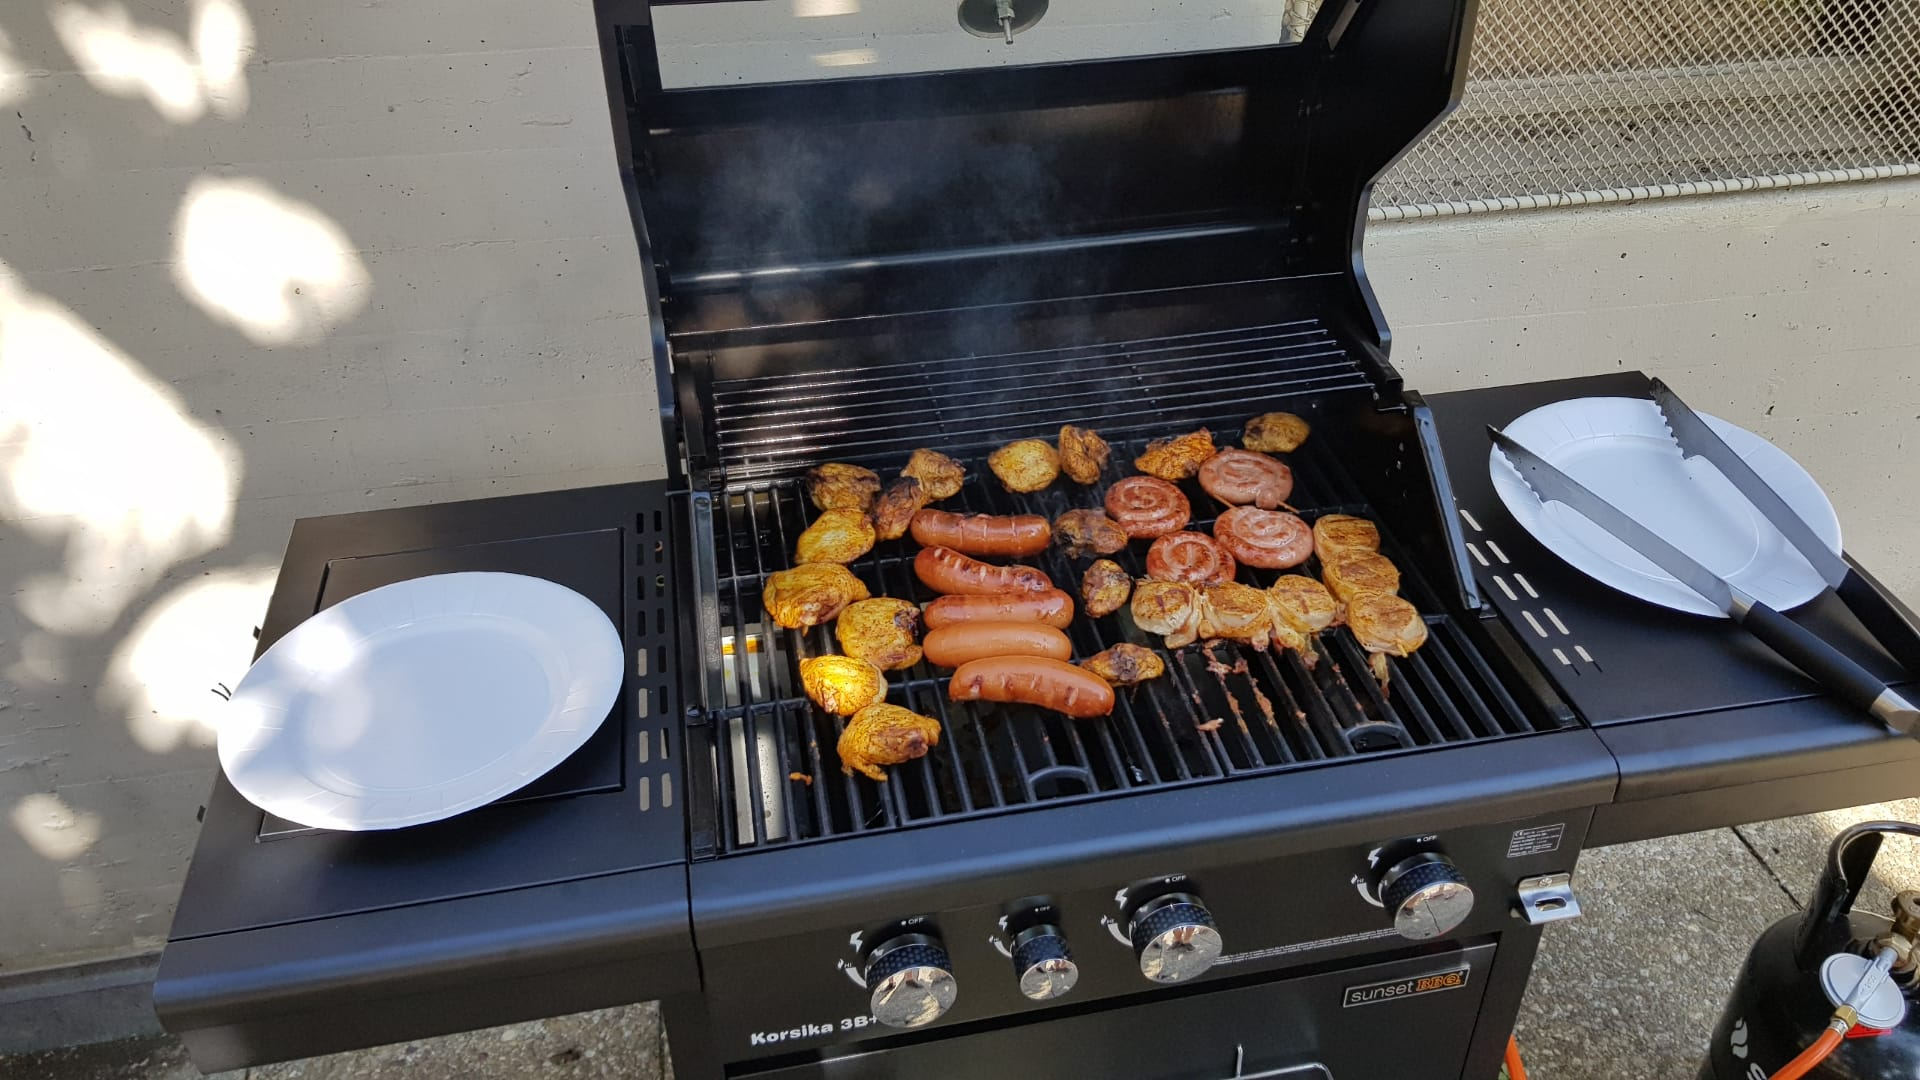
\includegraphics[width=0.9\linewidth]{Figures/Ack/korsika}
\end{center}

A mi hermano, porque aunque no hayamos tenido la mejor ni la más intensa de las relaciones, siempre se ha alegrado de todo lo que he conseguido y yo siempre estaré orgulloso de lo que él alcance.

A mis padres porque lo han dado todo para que nunca nos faltara de nada. Porque todo lo que ha estado en su mano ha sido para nosotros en lugar de para ellos. Porque siempre nos han tratado con cariño y comprensión. Porque gracias a ellos he podido ser todo lo que he querido.

\newpage

A Carol, porque apareció justo en el momento perfecto y yo no creo en las coincidencias. Ella ha soportado todo lo malo de este camino y lo ha amortiguado, ha recibido todo lo bueno y lo ha potenciado. Han sido muchos momentos difíciles para los dos en todos los sentidos y hemos compartido todas las preocupaciones e inquietudes que se le pueden pasar a uno por la cabeza. Han sido también los años más intensos de mi vida gracias a ti. No sé lo que nos deparará la vida, pero siempre tendrás un hueco en mi corazón. Eres la mejor compañera de viaje que uno puede imaginar.\\

\begin{center}
	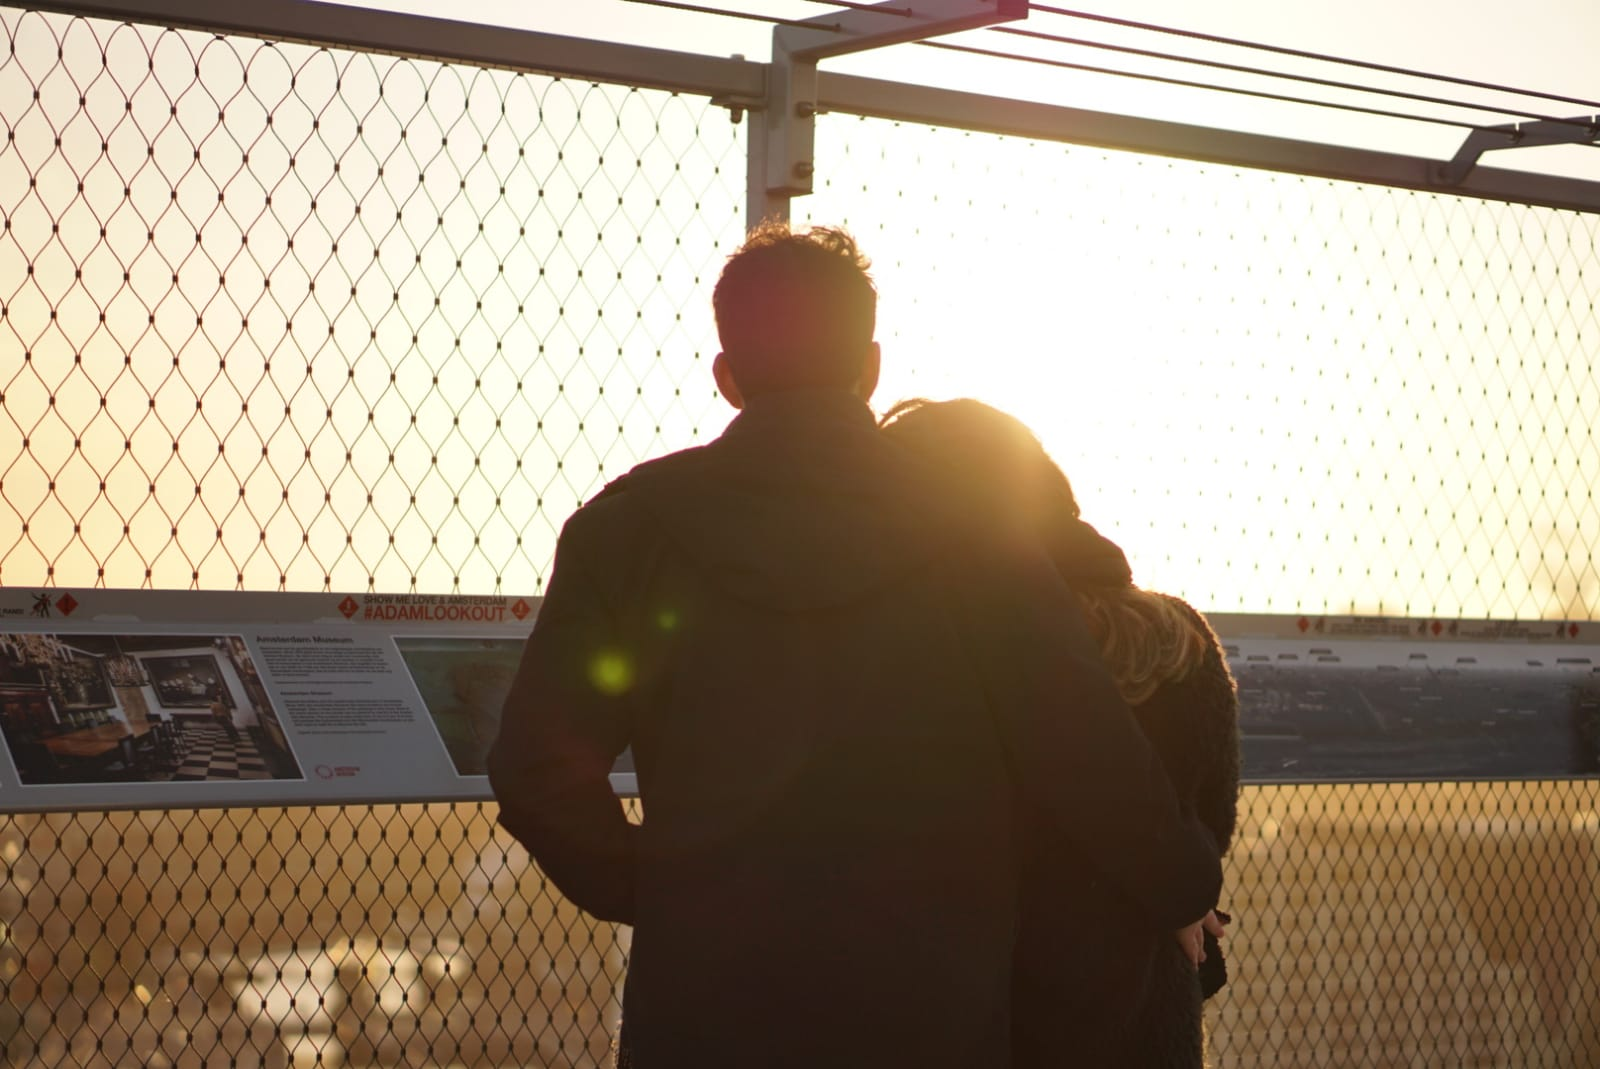
\includegraphics[width=0.9\linewidth]{Figures/Ack/carol}
\end{center}

\noindent\emph{Alberto García García}\\
\emph{Septiembre de 2019}\\
\emph{Zürich}\\

\vfill

\emph{Quisiera aprovechar estas líneas para agradecer al Gobierno de España (becas y proyectos FPU15/04516, DPI2013-40534-R, TIN2016-76515-R, GV/2018/022) por financiar todos estos años de estudios, estancias, viajes y oportunidades. También me gustaría agradecer a NVIDIA Corporation por sus generosas donaciones de hardware que permitieron desarrollar esta tesis.}\\

\chapter{Acknowledgements}

What does it feel like to look back? What goes through your head before turning the last page of a book that has trapped you for hours and hours? What's left when, at the top of the mountain, you look up only to discover that everything is under your feet? All the stories end somehow or other and all that's left when they do is the emptiness of knowing that nothing can ever replace them, or even come close to them. It is the inescapable sensation of everything that at the end of the road has been worthwhile.

This document gathers in an academic way the history of the best six years of my life. Behind all the technicalities is the history of more than twenty cities; of no less than sixty flights, trains and cars; and most importantly: of at least one hundred people. Unfortunately, I don't think any publisher with two fingers in front decided to publish such a nonsense, so I will take advantage of these pages that will be published without revision to tell my life.

Like any child fascinated by space, I am a frustrated astronaut. One who did not have the courage to move and study Physics and who fortunately had too sweaty hands to devote himself to Architecture. The eighty meter of my childhood made me a good basketball player until everyone grew up. The football goal, which will always be the place where I feel the most important person in the Universe, was at the same time too lonely for me. I played the piano without brilliance. I painted without genius. I wrote, published, but scarce in ink and imagination. I designed and built bridges, but only from ice cream sticks. I tried many things and was lucky enough to find my ikigai in computing. I guess the moment I installed my first graphics card and ran \verb|C:\DOOM\doom.exe| everything was sealed. I never imagined that the kid who just wanted to make a fun video game would end up spending countless hours devouring all the knowledge he could find about programming, data structures and algorithms.

So, like all my generation, I entered the University with the promise of a job and a dignified life earned through study. Thus, the best moments of my life took place between foosball games, worries and dream faces before entering class, laughs when leaving them and nights of eternal League of Legends and Counter Strike games. It has nothing to do with the person who came in (closed, short phrases and scarce smiles) with the one who came out (determined, talkative and smiling). By the way, I managed to dress a little more decently, although I still can't find a way to combine colors with success. In those four years I met a group of exceptional people, I learned and studied to the smallest detail, I met who would be my guide in the years to come and I discovered that research was my mission in life.

When I finished, I flew for the first time on my own to the Supercomputer Center in Jülich (Germany) for what would be my first stay abroad. They were undoubtedly the most transcendental moment in my life. I have such a good memory of those weeks that I never wanted to go back because I didn't want to spoil it. As Master Sabina would say: "[...] that to the place where you have been happy, you should not try to return [...]".

More out of inertia and illusion than logic, I decided to study a master's degree in Automation and Robotics at my alma mater. To be honest, it was not the smartest alternative for my future (not because of the master itself). Quite simply, over time I realized that deep down I will always regret not getting on an airplane to discover another university. However, if I hadn't stayed, I would never have met or befriended one of the best people I've ever met. Every time I think I should have flown, I remember him eating a whole lemon with skin and it passes.

As if my cries were somehow heard, life gave me the unbeatable opportunity to fly to the United States and do research at one of the companies I will be most fond of. So I ended up living in Mountain View (California) and working for NVIDIA with an exceptional team. They were months of discovery and will remain forever in my memory the memories of my small room in Villa Street, the bus driver to whom I never asked his name but who always took me with a smile to work and a "Hey, buddy!", the games of ping pong, the DeLorean parked in front of my house and enjoy the Olympic Games in the projector of the house of Cole shouting "USA, USA, USA! Cole and Grayson's hospitality made those months fly by.

As man is the only animal that stumbles twice on the same stone, I returned again to Alicante to begin my doctorate. Again, one of my biggest flaws played a trick on me and clouded my judgment in choosing: comfort. Again, there will always remain in my head the unknown of what would have happened if I had decided to stay in the United States instead of flying back. Again, as if some kind stranger helped me carry a heavy load, life would pat me on the back and remind me that it wasn't such a bad choice. Just a few weeks after my return, perhaps moved by the confidence breathed by all that had been achieved, perhaps guided by ethylic unconsciousness, I sent a message that allowed me to meet the person who has given me everything I lacked in life. Like a perfect Tetris, all the pieces began to fall into place: with the guidance and drive of my directors (more friends than bosses) and with the return of old colleagues we formed a team with which we managed to push the frontier of knowledge with a lot of effort but with the pride of a job well done despite all the obstacles. Once again, with fortune smiling, I left once again for the United States to work with one of the people I have most admired since I began my career. It was a complicated fall, with my head more dispersed than ever, and I left with the feeling that I had not done everything in my hand.

That scattered head spent a few more months lost and with the feeling of wasting time. The inevitable comparison with everyone around the globe was not favorable. The experiences lived, while enriching, were a double-edged sword capable of undermining one's self-confidence by realizing all the talent and exceptional people who work tirelessly outside. The prospect of the end of the stage added even more if possible a component of uncertainty which became a scarce dream, irritability, demotivation and pessimism. I became my own worst enemy, unable to feel satisfied with the past, completely alien to the present and blind to the future. Moving forward, seeking refuge in all the existing hobbies (many of which ended up becoming a fantastic decoration for my room) and only spurred on by the parallel studies in Physics and by the encouragement of loved ones to continue, I began to write the document I present here.

It was just at the moment of greatest discouragement in my career when something completely unexpected happened that changed everything. Without any gain or motivation, I left for Zurich to spend the summer months in what would be my last stay, again in Oculus. When I needed it most, all the stars lined up to offer me a fantastic city and house, an extremely capable and friendly team of people, an attentive and understanding mentor... and a group of people from my land tremendously close to whom to share absolutely everything. Thanks to that I regained the motivation and the illusion to go ahead and be able to write these lines.

As you can read, it has been a curious path full of ups and downs. This emotional roller coaster has cost me hair, hours of sleep, arguments and many regrets. However, now standing from the top of the mountain, looking at my life from a bird's eye view I can say that nothing would have changed. I have walked my own path all the honesty and integrity I could, I have put in all the effort my mental health has allowed me and I have tried to be the best version of myself at every step taken. Sometimes I will have succeeded and sometimes I will have failed, but this has been the path I have traced and that is something I will remember fondly all my life.
Before my eyes there are now countless summits that I could never have seen hidden by the clouds at great heights. Here I plant my flag and I feel to thank all those people who in one way or another have allowed me to get here.

Thanks to all those teachers who made an effort in their day to day life full of complications for their students to learn and who day to day showed us their affection and involvement. I am sure that if any of you from both Colegio Sagrada Familia and Colegio El Valle read these lines you will feel identified and go for you. Specifically, I would like to dedicate a few lines to thank an exceptional person who will always have my deepest admiration: Don Carlos. Beyond teaching us, he knew how to transmit passion, authenticity and affection to us even in the most difficult days. I cannot forget either Don Francisco, from whom I learned the importance of language; if one day I write a novel, it will be his fault.

Thanks to all the university professors who, surrounded by incompetence, obstacles and reluctance, continued to give everything they had to keep public education in the place it deserves. I would like to take this opportunity to thank José Miguel Torrejón for showing us that the difficult can be made easy with the right explanation and for always having his door open to any curiosity. In the same way to José Pons, for doing everything in his power so that he could train me in Physics and offer me a new opportunity to explore.

Thanks to all those who were my guide during my research stage. To Higinio because he is really responsible for me dedicating myself to research, thank you for your frankness, dedication and sincerity.

To Jose, for welcoming me and always treating me like a friend; even though you haven't been in the sand, you have fought for me and always tried to look for the best for my future even when the best for me wasn't the best for you; you haven't been my director, you've been my friend and academic father.

To Sergio, because without him everything would have been directly impossible; you have been with all of us always at the foot of the barrel no matter when or where, you have been the glue that has kept us together, the mirror in which we have all wanted to look and the source of inspiration that has pushed us all to be better every day.

To Ivo, because his energy is contagious and his optimism untiring. To David, although I can only say the opposite about him.

To my manager and mentors at NVIDIA, Howard, Bryan and Shalini, for all the time you gave me and the good treatment I received from you. To all the members of NVIDIA Research and the Camera Solutions team for sharing so much knowledge and advice: Orazio, Kihwan, Jinwei, Pavlo, Jan, Vidya, Dhaval and John. To all the interns who share so many good times, concerns and naps: Suren, Robert, Behrooz, Zhaopeng and Abhishek.

To my mentor during my stay at Facebook Reality Labs, Richard Newcombe, it was amazing for me to be able to share ideas with someone I admired so much, thank you for making room in your diary. To Raúl for making my stay easier. To Lingni for having so much patience with me, I've never seen anyone work so hard. To Svet for his calibration files. To the other teammates of Surreal and Oculus Research who made me feel at home: Nikki, Theo, Julian, Carl, Tom and Steve.

To the students with whom I have had the pleasure of sharing a few hours. Thank you for giving me your attention and affection. I never imagined that I would enjoy teaching so much but I can assure you that with you in the classroom I have shared some of the moments in which I have felt most full in life. Special thanks to all of you who decided to spend your time with me doing your TFG or internship: Álvaro, Adri, Alexei, Iván, Plácido, Mario, David and Pablo. Your curiosity and drive made me want to see you every day. I hope you all get everything you propose and share it with me wherever you go.

To all the famous people who have passed through the laboratory and who in one way or another have contributed their grain of sand to make the days different: Rafa, Marcelo, Jose María, Luis, Vicente, Alexandros, Zuri, Isaza, Alejandro, Pau, Toni, Jose Manuel... And to Joan Carles for giving my MAC address and teaching me how to play paddle.

To all the unforgettable companions that I have had the pleasure and luck to meet during the race, in the precise order in which I greeted each of them: Manu, 0xthor, Pajarraco, Márinero, Pable, Víctor, Ginés, Caye and last but not least, Brayan. Never again in my life will I find a group of people with whom I can share so many hobbies, laughs, cafés, sleepless nights and rusheos for B. Anything I could write here would fall short.

To my fellow island researchers: Pable, Sergiu and John. For demonstrating that when we row together without complaining we can do whatever we want and get to San Sebastian.

To my two companions of the Master: Victor and Fran. For all the sorrows and laughter shared in the most depressing and empty stage of my life. I doubt very much that I could have finished it without the synergy of these two great guys: an irreconducible nihilist and an unshakable bonachón.

To all the people in Zurich who made me regain my enthusiasm and motivation in my work. To my manager, Diego Tipaldi, for his kindness, understanding, his ability to rejoice in all the small victories and for his tireless effort to make the whole team feel at ease. To all the people from my team, the office and other parts of the world who came to my aid without a second thought: Chino, James, Amy, Jan, Alex Sorkine, Gaurav, Manuel, Alex Locher, Alexandru, Paul, Micky, Mahdi and Nikita. To the other interns who share many free dinners on Mondays and Thursdays: Katrin, Joao and Audrey. To all the recruiting team: Tanja for always being attentive to us, Oliver for always supplying cakes and Leslie for techno.

To the Spanish Mafia. We are responsible for making the months in Switzerland completely unforgettable. Thanks to Alejo, the main reason that he will arrive there, paddle master and wild card for all the parties. To Elena, for filling the office with plants. To Rubén, because things are more fun if you have someone touching your nose all day long. Fabrizio, although not Spanish, discovered the word ¨Maripepa¨. To Mariano, last of my shoe in the table of ping-pong, unfathomable philosopher and instigator of karaokes. To Berta, for imbuing the word "jodo" with so many meanings and for being my companion in songs and cocks. To Clara, for showing me that you can't miss class or eat at a barbecue. Special mention to my companion of building and breaks, Chema; well of wisdom, anecdotes and teachings. And finally, to that which united us, to our adopted daughter: the Korsika barbecue.

To my brother, because although we haven't had the best or the most intense of relationships, he has always been happy about everything I've achieved and I'll always be proud of what he achieves.

To my parents because they have given everything so that we would never lack anything. Because everything that has been in their hand has been for us instead of for them. Because they have always treated us with affection and understanding. Because thanks to them I have been able to be everything I wanted.

Carol, because she showed up at just the right time and I don't believe in coincidences. She has endured all the bad in this path and has cushioned it, she has received all the good and has empowered it. There have been many difficult moments for both of us in every way and we have shared all the concerns and worries that can pass through your head. They have also been the most intense years of my life thanks to you. I don't know what life will bring us, but you will always have a hole in my heart. You're the best travel companion you can imagine.\\

\noindent\emph{Alberto García García}\\
\emph{September, 2019}\\
\emph{Zürich}\\

\vfill

\emph{I want to thank the Government of Spain (grant programs FPU15/04516, DPI2013-40534-R, TIN2016-76515-R, GV/2018/022) for funding these years of research, internships and attendances to international conferences. I also gratefully acknowledge the support of NVIDIA Corporation with the donation of hardware used for this research.}\\

\chapter{Disacknowledgements}

This brief paragraph here is a reflection originally written by my colleague Mariano Jaimez Tarifa. It is a thought that I believe captures to perfection the feelings of every single researcher in Spain. Let this "disacknowledgement" serve as a way to raise awareness about our despicable political leaders and the rottenness of an education system full of incompetent and dishonest professors.

\emph{"The Government of Spain has invested a significant sum of money in this thesis during a period when the Spanish economy was in crisis. Unfortunately this investment is not going to be profitable for the Spanish State because the lack of a powerful technological industry in our country pushes me to seek for jobs abroad. I sincerely feel this is a pitty and a detrimental situation for Spain but it is not in my hands to change it. The Spanish government should promote a much tighter collaboration between companies and researchers in order to avoid this. How to do that in an efficient way is beyond my knowledge, but it might be worth thinking about all the work developed by hundreds of PhD students which falls into oblivion after they finish. I believe that huge amount of effort deserves a better fate."}


